%% Slides for ".NET Programming" by Chunyu Wang <chunyu@hit.edu.cn>
%% $Rev$

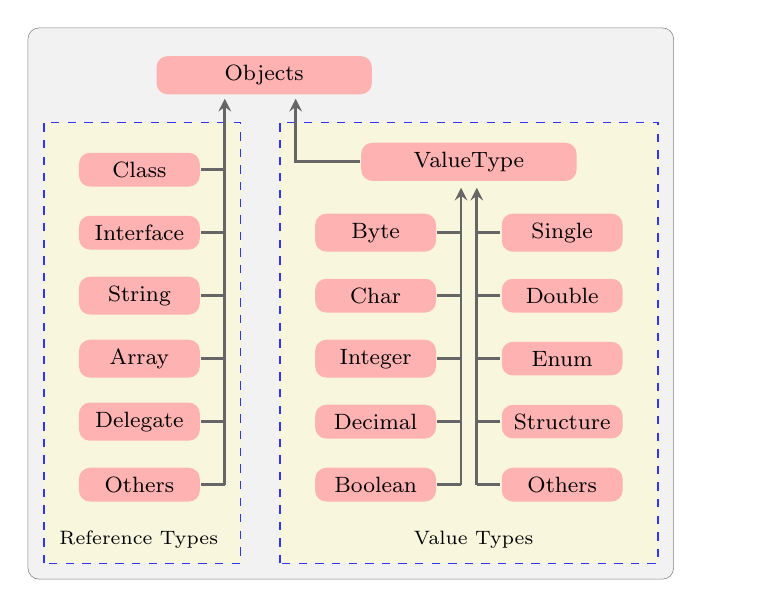
\begin{tikzpicture}[line width=1pt, >=stealth, draw=black!60]
\tikzstyle{every_node}=[font=\color{black}\footnotesize, text width=1.3cm, text centered, fill=red!30, rounded corners]
\tikzstyle{nnnn}=[anchor=center, text width=4cm, font=\color{black}\scriptsize]
\filldraw[fill=gray!10, draw=gray, line width=.2pt, rounded corners] (-.2,.8)  rectangle +(8.2, 7);

\filldraw[anchor=center] (2.8,7.2) node[style=every_node,text width=2.5cm] {Objects};

\filldraw[fill=yellow!20, fill opacity=.5, line width=.6pt,draw=blue!80, dashed] (0,1) rectangle +(2.5,5.6);
\filldraw[fill=yellow!20, fill opacity=.5, line width=.6pt,draw=blue!80, dashed] (3,1) rectangle +(4.8,5.6);
\filldraw (2.2, 1.3) node[style=nnnn] {Reference Types};
\filldraw (6.7, 1.3) node[style=nnnn] {Value Types};

\filldraw[anchor=center] (5.4,6.1) node[style=every_node,text width=2.5cm] (vt) {ValueType};
\draw[->] (vt) -| (3.2,6.9);

\foreach \a/\b in {2/Others,2.8/Delegate,3.6/Array,4.4/String,5.2/Interface,6/Class}
{\filldraw (2, \a ) node[style=every_node,anchor=east] {\b};
  \draw (2, \a ) -- (2.3, \a );}
\draw[->] (2.3,2) -- (2.3,6.9);
\foreach \a/\b in {2/Boolean,2.8/Decimal,3.6/Integer,4.4/Char,5.2/Byte}
{\filldraw (5, \a ) node[style=every_node,anchor=east] {\b};
  \draw (5, \a ) -- (5.3, \a );}
\draw[->] (5.3,2) -- (5.3,5.77);
\foreach \a/\b in {2/Others,2.8/Structure,3.6/Enum,4.4/Double,5.2/Single}
{\filldraw (5.8, \a ) node[style=every_node,anchor=west] {\b};
  \draw (5.8, \a ) -- (5.5, \a );}
\draw[->] (5.5,2) -- (5.5,5.77);
\end{tikzpicture}
